\subsection{Dobozmodell}

%30
\begin{frame}
  \begin{columns}[c]
    \column{0.5\textwidth}
      Minden HTML elemet egy \emph{doboznak} tekintünk. Ezek szerkezete belülről kifelé:
      \begin{itemize}
        \item Az elem tartalma (szöveg, kép, \dots)
        \item Kitöltés (\texttt{padding}; átlátszó)
        \item Szegély (\texttt{border})
        \item Margó (\texttt{margin}; átlátszó)
      \end{itemize}
      \vfill
      Megjegyzések
      \begin{itemize}
        \item A szélesség (\texttt{width}) és magasság (\texttt{height}) 
      tulajdonságok a tartalmi rész méreteire vonatkoznak.
        \item Soron belüli elemek méretét a böngésző határozza 
        meg, nem méretezhetőek át.
      \end{itemize}
    \column{0.5\textwidth}
      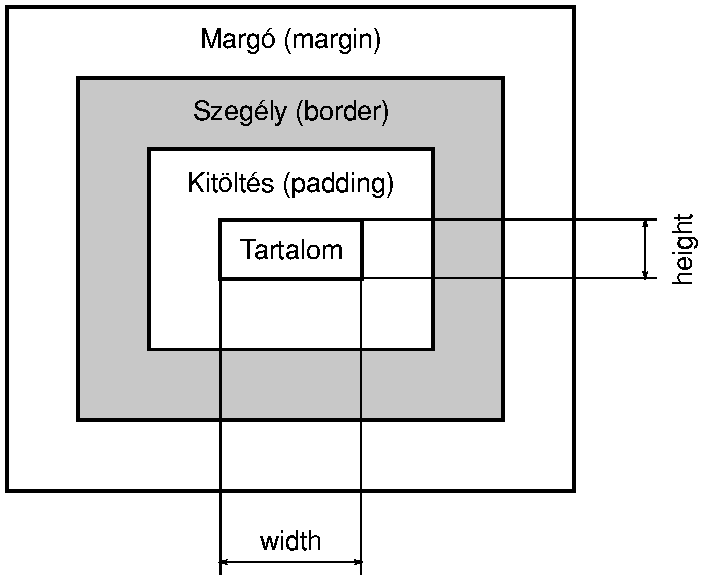
\includegraphics[width=\textwidth]{doboz.pdf}
  \end{columns} 
\end{frame}

%31
\begin{frame}
  \begin{columns}[c]
    \column{0.45\textwidth}
      \begin{exampleblock}{\textattachfile{dobozMeret.html}{dobozMeret.html}}
        \tiny
        \lstinputlisting[style=HTML,linerange={7-18},numbers=left,firstnumber=7]{dobozMeret.html}
      \end{exampleblock}
    \column{0.55\textwidth}
      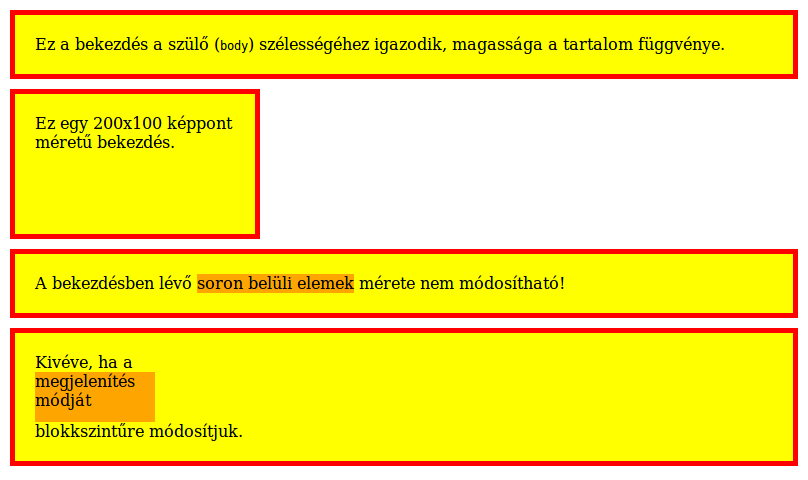
\includegraphics[width=0.9\textwidth]{dobozMeret.png}
  \end{columns}
  \begin{exampleblock}{\vspace*{-3ex}}
    \tiny
    \lstinputlisting[style=HTML,linerange={22-25},numbers=left,firstnumber=22]{dobozMeret.html}
  \end{exampleblock}
\end{frame}

%32
\begin{frame}
\begin{columns}[c]
  \column{0.5\textwidth}
    Mit számol bele a böngésző a méret (\texttt{width}, 
    \texttt{height}) adatokba? $\to$ \texttt{box-sizing}
    \begin{description}[m]
      \item[\texttt{content-box}] \hfill \\ 
        Csak a tartalom méretét
      \item[\texttt{border-box}] \hfill \\ 
        Tartalom + kitöltés + szegély
    \end{description}
    \vfill
    Kényelmes:\\
    \texttt{* \{ box-sizing: border-box; \} }
  \column{0.5\textwidth}
    \begin{center}
      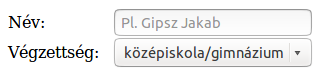
\includegraphics[scale=0.5]{meretezes.png}
    \end{center}
    \begin{exampleblock}{\textattachfile{meretezes.html}{meretezes.html}}
      \scriptsize
      \lstinputlisting[style=HTML,linerange={11-17},numbers=left,firstnumber=11]{meretezes.html}
    \end{exampleblock}
\end{columns} 
\end{frame}

%33
\begin{frame}
  Blokk szintű elemek szélessége (\texttt{width}) és magassága (\texttt{height}) megadható:
  \begin{itemize}
    \item \texttt{auto}: alapértelmezett
    \item valós világbeli, relatív vagy megjelenítőtől függő mértékegység (pl. \texttt{cm}, \texttt{ex}, \texttt{px})
    \item a tartalmazó blokk \%-ában megadva
    \item Érdekes lehetőség az abszolút és relatív méretek vegyítésére: \texttt{calc()} függvény. Négy alapműveletes kifejezések kiértékelhetők vele.
  \end{itemize}
\end{frame}

%_
\begin{frame}
  \begin{columns}[c]
    \column{0.66\textwidth}
      \begin{exampleblock}{\textattachfile{calc.html}{calc.html}}
        \scriptsize
        \lstinputlisting[style=HTML,linerange={7-11},numbers=left,firstnumber=7]{calc.html}
        \lstinputlisting[style=HTML,linerange={14-16},numbers=left,firstnumber=14]{calc.html}
      \end{exampleblock}
    \column{0.3\textwidth}
      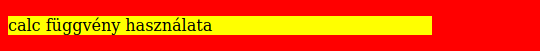
\includegraphics[width=\textwidth]{calc.png}
  \end{columns}
\end{frame}

%34
\begin{frame}
  A merev méretek helyett megadhatók intervallumok is:
  \begin{description}[m]
    \item[\texttt{max-width}] \hfill \\ Ennél csak keskenyebb lehet. Felülírja \texttt{width} értékét.
    \item[\texttt{min-width}] \hfill \\ Ennél csak szélesebb lehet. Ha a tartalom ennél szélesebb, nem veszik figyelembe. A szélesség változásával a magasság is változhat.
    \item[\texttt{max-height}] \hfill \\ Ennél csak alacsonyabb lehet. Ha a tartalom ennél magasabb, a viselkedés az \texttt{overflow}-tól függ. Felülírja \texttt{height} értékét.
    \item[\texttt{min-height}] \hfill \\ Ennél csak magasabb lehet. Ha a tartalom ennél alacsonyabb, akkor ekkorára növeli meg a magasságot.
  \end{description}
\end{frame}

%35
\begin{frame}
  Túlcsordulások kezelése: \texttt{overflow}
  \begin{description}[m]
    \item[\texttt{visible}] \hfill \\ A túllógó részek is megjelennek, esetleg rálógva más tartalmakra. Alapértelmezés.
    \item[\texttt{hidden}] \hfill \\ A túllógó részeket levágják.
    \item[\texttt{scroll}] \hfill \\ Görgetősávok jelennek meg a túllógó részek megjelenítéséhez. Némelyik böngésző mindig mutatja, mások csak akkor, ha szükséges.
    \item[\texttt{auto}] \hfill \\ Csak akkor jelennek meg görgetősávok, ha nem fér el a tartalom.
  \end{description}
  \vfill
  Léteznek \texttt{overflow-x} és \texttt{overflow-y} tulajdonságok csak az egyik irány viselkedésének megadásához.
\end{frame}

%36
\begin{frame}
  \begin{exampleblock}{\textattachfile{tulnyulas.html}{tulnyulas.html} -- Ellenőrizze a méretezés hatását, túlcsordulásokat!}
    \scriptsize
    \lstinputlisting[style=HTML,linerange={11-12},numbers=left,firstnumber=11]{tulnyulas.html}
    \lstinputlisting[style=HTML,linerange={20-22},numbers=left,firstnumber=20]{tulnyulas.html}
  \end{exampleblock}
  \begin{columns}[T]
    \column{0.5\textwidth}
      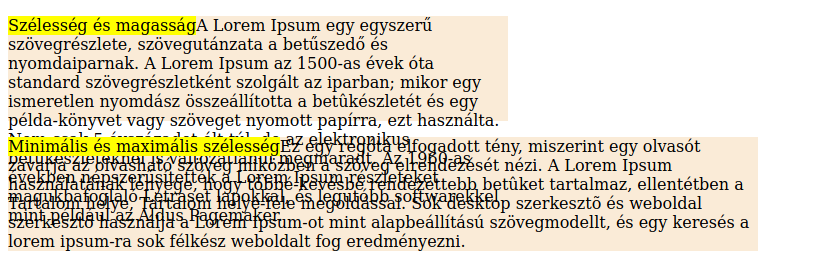
\includegraphics[width=\textwidth]{tulnyulas.png}
    \column{0.45\textwidth}
      Az első bekezdés tartalma rálóg a másodikra, túl alacsony a blokk.\\
      A második bekezdés maximális méreten. Ha keskenyre állítjuk az ablakot, vízszintes görgetősáv jelenik meg a böngészőablak alján.
  \end{columns}
\end{frame}
